\chapter{Gestion du projet}
\section{Équipe projet}
Notre équipe projet se compose de 4 personnes aux bagages et compétences (hors cursus Telecom ParisTech) complémentaires et équilibrés :
\begin{itemize}
\item \textbf{Charles Thérond} : fort d'un master en Machine Learning, Charles possède une bonne expérience en Python et R avec une connaissance pointue des outils et packages de data visualisation. Charles connaît les développements en méthodes agiles et a eu l'occasion d'implémenter des systèmes de gestion Big Data avec  Spark/Hadoop.
\item \textbf{Ioan Catana} : avec une solide expérience professionnelle chez Oracle, Ioan dispose des connaissances approfondies en bases de données, ainsi qu'en virtualisation et scripts Bash, Shell et Perl. Ioan a également eu l'occasion de mettre en oeuvre des interfaces de visualisation en R avec le package Shiny.
\item \textbf{Karine Pétrus} : avec son expérience de recherche au Laboratoire des Sciences du Climat et de l'environnement du CNRS, Karine dispose d'un solide bagage scientifique en Géo-Science, qui l'a amenée à manipuler des méthodes de traitement du signal en lien avec les phénomènes météorologiques.
\item \textbf{Stéphane Mulard} : après 5 ans de développement d'applications Web et 10 ans de conseil en systèmes d'information, Stéphane a acquis une solide expérience sur les problématiques d'architecture du SI, de modélisation de données et de gestion de projet en mode agile.
\end{itemize}

\section{Organisation du travail}
\subsection{Nos interlocuteurs}
Notre équipe projet travaille en étroite collaboration avec nos référents, au travers de points d'avancement réguliers et d'outis collaboratifs spécifiques :

\textbf{Notre référent académique Télécom ParisTech} : Stéphan Clémençon
\begin{itemize}
\item Réunions et points d'avancement réguliers
\item Orientations techniques
\end{itemize}

\textbf{Notre encadrant Engie} :  Paul Poncet
\begin{itemize}
\item Cadrage du projet
\item Réunions toutes les 15 jours (présentielles ou Skype)
\item Création d’un repository Github pour partager les développements
\item Création d’une chaîne dédiée Slack
\item Signature d’un accord de confidentialité
\end{itemize}

\subsection{Les outils collaboratifs et principes de travail}
Afin d'organiser le projet de façon efficace, nous avons mis en place plusieurs outils de travail collaboratif au sein de l'équipe :

\textbf{Outils Google Drive} : il s'agit de nos outils de travail principaux pour ce qui est de l'organisation de nos tâches, du planning, des ressources documentaires ou encore de l'historique du projet. On peut citer principalement :
\begin{itemize}
\item \emph{Tableau de bord de pilotage} : un résumé des tâches en cours, à réaliser ou terminées, assignées à chacun de nous, avec des dates de début et de fin.
\item \emph{Plan projet Gantt} : le fichier de planning global en cohérence avec notre liste de tâches.
\item \emph{Base de ressources documentaires} : une liste qualifiée des ressources documentaires que nous avons compulsées, avec leur difficulté technique, leur pertinence par rapport au projet et une brève description.
\item \emph{Modèles de documents} : comptes rendus de réunion, journal, table des matières du rapport, etc.
\end{itemize}

\textbf{Outil de gestion de source} :
\begin{itemize}
\item Repository Github
\end{itemize}

\textbf{Outil de rapport} :
\begin{itemize}
\item Overleaf : logiciel permettant le travail collaboratif pour l'édition de documents au format Latex et dispose d'un lien avec Github.
\end{itemize}

\textbf{Principes d'organisation agiles} : nous avons adopté plusieurs principes inspirés des méthodes agiles pour organiser le travail.
\begin{itemize}
\item Une définition des formats de travail
\item Des "sprints" de deux semaines avec des objectifs que l'équipe peut consulter à tout moment et des points d’avancement réguliers.
\item Travail en binômes : des séances de travail en binôme, notamment pour le codage (peer-coding).
\end{itemize}

\section{Choix techniques}
\textbf{Développement} : nous livrerons du code en langage Python, via des Notebook Jupyter, ou des fichiers .py. En effet l'équipe Engie a l'habitude de travailler avec ce langage, notamment en phase de prototypage.

\textbf{Plateformes} : Le volume de données que nous allons traiter est raisonnable (quelques gigaoctets). Ce qui nous permet de travailler sur nos machines personnelles. Si le besoin s'en fait sentir nous pourrons également accéder à des poste Engie disposant de 32 Mo de RAM, voire accéder à la plateforme de calcul Teralab de TelecomParisTech, mais à priori cela ne sera pas nécessaire.

Pour ce qui est des packages, nous avons identifié la liste suivante qui évoluera certainement au cours du projet :

\begin{figure}[!ht]
\begin{center}
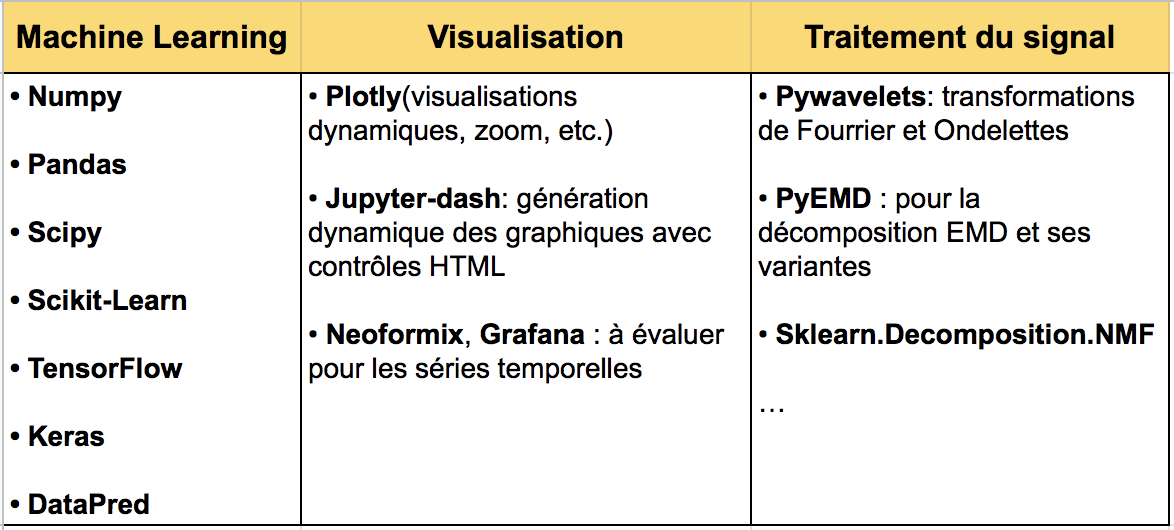
\includegraphics[scale=0.6]{rapport/images/Ch2_Packages.png}
\end{center}
\caption{Packages identifiés}
\end{figure}

\section{Analyse des risques}
Nous avons réalisé une analyse des risques initiaux illustrés dans le tableau ci-dessous. Pour chaque risque nous avons évalué une probabilité d'occurrence, un impact potentiel ainsi que des mesures d'atténuation. Comme le projet lui-même est voué à évoluer au cours des prochains mois, cette analyse sera revue lors de la prochaine soutenance.

\begin{figure}[!ht]
\begin{center}
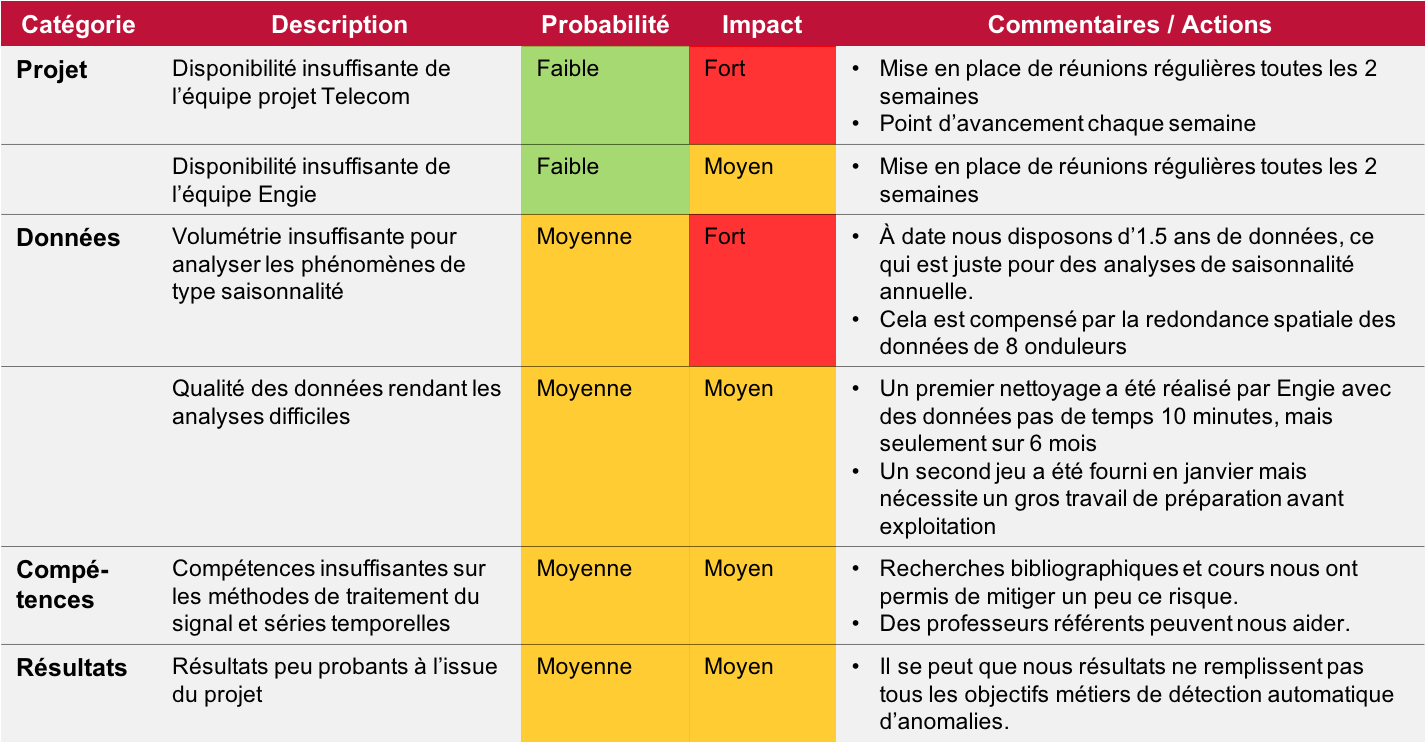
\includegraphics[scale=0.5]{rapport/images/Ch2_AnalyseRisques.png}
\end{center}
\caption{Analyse des risques}
\end{figure}

\section{Planning prévisionnel}
À date le planning prévisionnel que nous avons établi est le suivant, en cohérence avec les étapes de notre approche méthodologique (voir chapitre 4). Il faut bien noter que le déroulement du projet n'est pas linéaire et que nous ferons de nombreux allers-retours entre les étapes clés du projet (décomposition, identification des signatures, validation).

\begin{figure}[!ht]
\begin{center}
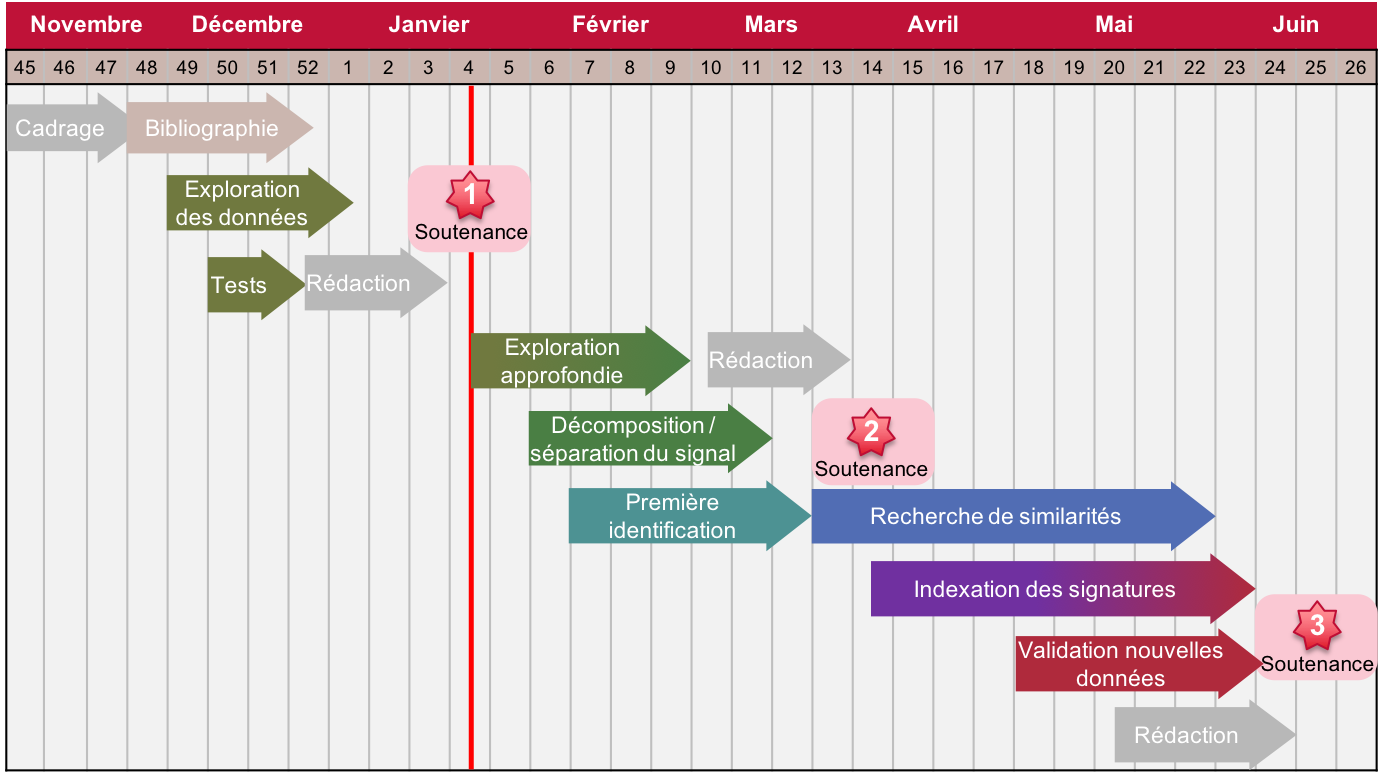
\includegraphics[scale=0.5]{rapport/images/Ch2_Planning.png}
\end{center}
\caption{Planning prévisionnel}
\end{figure}

\section{Répartition des tâches}
Définir la répartition des tâches est un exercice relativement difficile à ce stade du projet. Néanmoins nous l'avons réalisé, au moins en ce qui concerne les premières étapes du projet. Pour la suite, comme cela est illustré ci-dessous, nous privilégierons le travail en binômes.


\begin{figure}[!ht]
\begin{center}
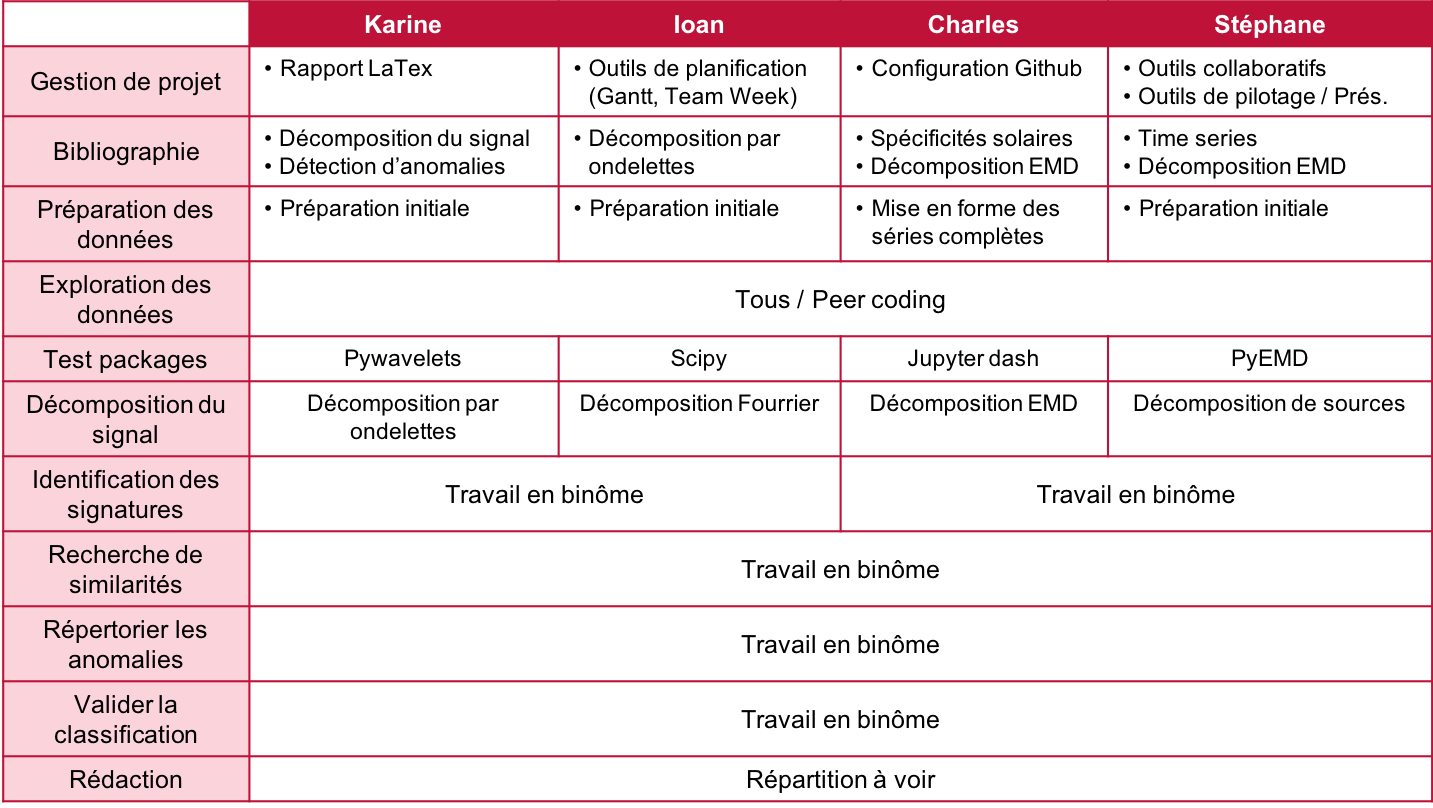
\includegraphics[scale=0.5]{rapport/images/Ch2_RepartitionTaches.png}
\end{center}
\caption{Répartition des tâches}
\end{figure}


